\section{Phonons into films}\label{sec:20.3}

A phonon that has down-converted in silicon to about a terahertz (\cref{sec:20.2}) reaches an aluminum film \SI{60}{nm} thick on the crystal surface. Silicon and aluminum have almost the same acoustic impedance, and the normal-incidence law of \cref{app:C.18} lets \SI{99}{\percent} of a longitudinal flux through. A fit of measured pulses with a phonon simulation nevertheless returns a silicon-to-aluminum coefficient of 0.3 to 0.55 for such a film~\cite{martinez2019measurements}, and a phonon inside the film that reaches the interface crosses back into the silicon about once in three arrivals. These three numbers measure different things. The transmission of each polarization at every angle, and the reciprocity that ties the two directions together, explain all three, and from them follow the probability that a phonon entering the film is absorbed there and the time $t_l$ it spends in the film before escaping, which controls the quasiparticle yield of \cref{sec:20.4}.

\subsection{Acoustic mismatch at oblique incidence}\label{sec:20.3-amm}

The acoustic mismatch model treats the interface as a welded plane between two elastic continua: displacement and traction are continuous across it, and nothing else happens there~\cite{swartz1989thermal}. Silicon is cubic, with an anisotropy ratio $2C_{44}/(C_{11} - C_{12}) = 1.56$ (\cref{app:C.18}). Aluminum is nearly isotropic: its elastic constants extrapolated to zero temperature, $C_{11} = 114.3$, $C_{12} = 61.9$ and $C_{44} = \SI{31.6}{GPa}$~\cite[Table~2]{malica2020quasi}, give the ratio 1.21. We replace each crystal by an isotropic medium with the Voigt averages of its elastic constants, the bulk modulus $B$ of \cref{eq:C.18-bulk} and the shear modulus $(C_{11} - C_{12} + 3C_{44})/5$, which is also what transport codes do. Silicon then has the speeds $c_{\mathrm{LA}} = \SI{9.00}{km.s^{-1}}$ and $c_{\mathrm{T}} = \SI{5.40}{km.s^{-1}}$ at $\rho_T = \SI{2.33}{g.cm^{-3}}$, and aluminum $c_{\mathrm{LA}} = \SI{6.63}{km.s^{-1}}$ and $c_{\mathrm{T}} = \SI{3.30}{km.s^{-1}}$ at the room-temperature density \SI{2.70}{g.cm^{-3}}. A subscript 1 or 2 on a speed or density names the medium.

Put the interface at $z = 0$, with medium 1 below it. A plane wave of frequency $\omega$ that arrives from medium 1 at the angle $\theta_1$ to the normal has the wavevector component $Q_\parallel = \omega\sin\theta_1/c_{\mathrm{inc}}$ along the interface, where $c_{\mathrm{inc}}$ is its speed. Every reflected and transmitted wave it generates has the same $\omega$ and the same $Q_\parallel$, which is the acoustic Snell law \cref{eq:C.18-snell}. A wave of speed $c$ in either medium then has the normal component
\begin{equation}
  Q_z = \bigl(\omega^2/c^2 - Q_\parallel^2\bigr)^{1/2} ,
  \label{eq:20.3-Qz}
\end{equation}
taken positive. When $Q_\parallel > \omega/c$ the root is imaginary, we take it with a positive imaginary part, and the wave decays away from the interface and carries no energy flux. A wave can have three polarizations: longitudinal (L), transverse in the plane of incidence (SV), and transverse perpendicular to it (SH). The interface is invariant under reflection through the plane of incidence, so SH waves couple only to SH waves, while L and SV waves mix.

For SH waves the displacement $u_y$ and the traction $\sigma_{yz} = \rho_Tc_{\mathrm{T}}^2\,\partial_zu_y$ must be continuous. This is the algebra of the normal-incidence derivation in \cref{app:C.18}, with $Q_i\rho_ic_i^2$ there replaced by $\rho_ic_{\mathrm{T},i}^2Q_{z,i} = \omega Z^{\mathrm{T}}_{\mathrm{ac},i}\cos\theta_i$, where $Z^{\mathrm{T}}_{\mathrm{ac},i} = \rho_ic_{\mathrm{T},i}$ is the transverse impedance. The fraction of the incident energy flux that crosses is
\begin{equation}
  t_{\mathrm{SH}}(\theta_1) = \frac{4Z^{\mathrm{T}}_{\mathrm{ac},1}\cos\theta_1\,\Real\bigl(Z^{\mathrm{T}}_{\mathrm{ac},2}\cos\theta_2\bigr)}{\bigl|Z^{\mathrm{T}}_{\mathrm{ac},1}\cos\theta_1 + Z^{\mathrm{T}}_{\mathrm{ac},2}\cos\theta_2\bigr|^2} ,
  \qquad
  \cos\theta_2 = \Bigl(1 - \frac{c_{\mathrm{T},2}^2}{c_{\mathrm{T},1}^2}\sin^2\theta_1\Bigr)^{1/2} .
  \label{eq:20.3-SH}
\end{equation}
At normal incidence it is \cref{eq:C.18-transmission} with the transverse impedances. Beyond the critical angle $\sin\theta_1 = c_{\mathrm{T},1}/c_{\mathrm{T},2}$, which exists when medium 2 is the faster one, $\cos\theta_2$ is imaginary and $t_{\mathrm{SH}} = 0$: the wave is totally reflected.

For L and SV waves four conditions hold at $z = 0$: continuity of $u_x$, $u_z$, $\sigma_{zz} = \rho_T[c_{\mathrm{LA}}^2\partial_zu_z + (c_{\mathrm{LA}}^2 - 2c_{\mathrm{T}}^2)\partial_xu_x]$ and $\sigma_{xz} = \rho_Tc_{\mathrm{T}}^2(\partial_zu_x + \partial_xu_z)$, the last two being Hooke's law of \cref{app:C.18} for an isotropic medium. Each wave is $u = a\,\hat{\vect{e}}\,\ee^{\ii(Q_\parallel x \pm Q_zz - \omega t)}$ with amplitude $a$ and the sign $+$ for a wave moving toward medium 2 and $-$ for one moving back into medium 1, and unit polarization $\hat{\vect{e}} = (c/\omega)(Q_\parallel, 0, \pm Q_z)$ for L and $(c/\omega)(\pm Q_z, 0, -Q_\parallel)$ for SV. Collect for each wave the four quantities that must match,
\begin{equation}
  \vect{b} = \Bigl(\hat e_x,\ \hat e_z,\ \frac{\rho_T}{\omega}\bigl[c_{\mathrm{LA}}^2(\pm Q_z)\hat e_z + (c_{\mathrm{LA}}^2 - 2c_{\mathrm{T}}^2)Q_\parallel\hat e_x\bigr],\ \frac{\rho_Tc_{\mathrm{T}}^2}{\omega}\bigl[(\pm Q_z)\hat e_x + Q_\parallel\hat e_z\bigr]\Bigr) ,
  \label{eq:20.3-b}
\end{equation}
which are the displacement and $\sigma_{zz}/\ii\omega$, $\sigma_{xz}/\ii\omega$ per unit amplitude. With unit incident amplitude the boundary conditions read $\vect{b}_{\mathrm{inc}} + a_{\mathrm{rL}}\vect{b}_{\mathrm{rL}} + a_{\mathrm{rS}}\vect{b}_{\mathrm{rS}} = a_{\mathrm{tL}}\vect{b}_{\mathrm{tL}} + a_{\mathrm{tS}}\vect{b}_{\mathrm{tS}}$, four linear equations for the amplitudes of the reflected (r) and transmitted (t) L and SV waves. A propagating plane wave carries the time-averaged energy flux $\frac12\rho_T\omega^2|a|^2c$ along its direction (\cref{app:C.18}), whose normal component is this times $\cos\theta = cQ_z/\omega$. The fraction of the incident flux carried away by the outgoing wave $j$ is therefore
\begin{equation}
  t_j = \frac{\rho_jc_j^2\,\Real Q_{z,j}\,|a_j|^2}{\rho_1c_{\mathrm{inc}}^2\,Q_{z,\mathrm{inc}}} ,
  \label{eq:20.3-flux}
\end{equation}
and the transmission of an incident L or SV wave is the sum of the two transmitted fractions. We solve the four equations numerically at each angle.

\Cref{fig:20-amm} shows the result for silicon and aluminum. From the silicon side, a longitudinal phonon crosses with 0.99 at normal incidence and with more than 0.98 out to \SI{70}{\degree}, falling below 0.9 only beyond \SI{78}{\degree}. At oblique incidence part of the transmitted flux is converted to SV, \num{0.031} at \SI{30}{\degree} and at most 0.17, near \SI{76}{\degree}. Transverse phonons cross with 0.97 at normal incidence. The one critical angle that limits transmission from silicon is \SI{54.6}{\degree}, beyond which an incident SV wave can no longer produce a longitudinal wave in aluminum. From the aluminum side, however, every wave is slower than every wave in silicon, and the critical angles cut transmission off. Transverse phonons beyond $\arcsin(c_{\mathrm{T,Al}}/c_{\mathrm{T,Si}}) = \SI{37.7}{\degree}$ find no propagating wave in silicon and are totally reflected. Longitudinal phonons lose the longitudinal channel beyond \SI{47.5}{\degree} and keep only the conversion into silicon transverse waves, which carries 0.28 at that angle and vanishes at grazing incidence.

\begin{figure}[tbp]
  \centering
  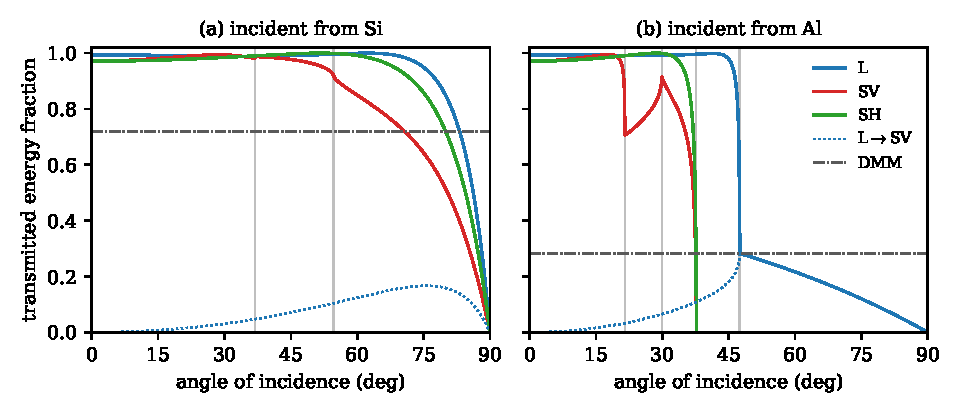
\includegraphics[width=\linewidth]{figures/ch20/fig20_3.pdf}
  \caption{Acoustic-mismatch transmission of a welded silicon/aluminum interface against the angle of incidence, for phonons incident (a) from silicon and (b) from aluminum. Solid: fraction of the incident energy flux transmitted into all modes of the other side, for incident longitudinal (L, blue), SV (red) and SH (green) phonons; dotted: the part of the incident longitudinal flux transmitted as SV. Dash-dot: the diffuse-mismatch value $\mathfrak{n}_2/(\mathfrak{n}_1 + \mathfrak{n}_2)$, 0.718 in (a) and 0.282 in (b). Gray lines: critical angles, \SI{36.9}{\degree} and \SI{54.6}{\degree} in (a); \SI{21.5}{\degree}, \SI{29.9}{\degree}, \SI{37.7}{\degree} and \SI{47.5}{\degree} in (b). Both media isotropic, with the Voigt averages of the elastic constants: silicon (\cref{app:C.18}) $c_{\mathrm{LA}} = 9.00$, $c_{\mathrm{T}} = \SI{5.40}{km.s^{-1}}$, $\rho_T = \SI{2.33}{g.cm^{-3}}$; aluminum, zero-temperature elastic constants at the room-temperature density, 6.63, \SI{3.30}{km.s^{-1}}, \SI{2.70}{g.cm^{-3}}. The curves do not depend on frequency.}
  \label{fig:20-amm}
\end{figure}

Frequency drops out of \cref{eq:20.3-SH,eq:20.3-flux}, because $Q_\parallel$ and $Q_z$ both scale with $\omega$. The transmissions are frequency independent as long as the wavelength is long compared with the lattice spacing, so that the continuum holds, and short compared with the film thickness, so that the film acts as a half-space. In the simulation of the \SI{60}{nm} films the absorbed phonons peak between 0.7 and \SI{0.9}{THz}~\cite[Sect.~V]{martinez2019measurements}. At \SI{0.8}{THz} the wavelengths in aluminum are \SI{8.3}{nm} for longitudinal and \SI{4.1}{nm} for transverse phonons, so both conditions hold. The longitudinal wavelength equals the thickness at \SI{0.110}{THz}, close to the pair-breaking threshold $2\Delta_{\mathrm{BCS}} = \SI{0.36}{meV}$, or \SI{0.087}{THz}, of bulk aluminum (\cref{sec:7.2}); below it the film reflects as a layer, with interference between its two faces.

\subsection{Angle averages, reciprocity and diffuse mismatch}\label{sec:20.3-recip}

A sensor film collects phonons arriving from all directions, so its transmission is the average over an isotropic population. Count the energy flux that such a population sends onto unit area of the interface. A branch has $\dd^3Q/(2\pi)^3$ modes in $\dd^3Q$, each with occupation $n(\omega)$, energy $\omega$ and normal group velocity $\partial\omega/\partial Q_z$. Since $\dd Q_z\,\partial\omega/\partial Q_z = \dd\omega$, the flux is
\begin{equation}
  \int_{Q_z > 0}\frac{\dd^3Q}{(2\pi)^3}\,\omega\,n(\omega)\,\frac{\partial\omega}{\partial Q_z} = \int\dd\omega\,\omega\,n(\omega)\int\frac{\dd^2Q_\parallel}{(2\pi)^3} .
  \label{eq:20.3-count}
\end{equation}
At a given frequency, every patch $\dd^2Q_\parallel$ of every branch, in either medium, brings the same flux. In an isotropic medium $\dd^2Q_\parallel = 2\pi Q_\parallel\dd Q_\parallel = (2\pi\omega^2/c_\nu^2)\sin\theta\cos\theta\,\dd\theta$, so the angles enter with the weight $2\sin\theta\cos\theta$ and the branch $\nu$ with the weight $c_\nu^{-2}$. The mean transmission of an isotropic population from medium 1 into medium 2 is
\begin{equation}
  \bar t_{12} = \frac{1}{\mathfrak{n}_1}\sum_\nu c_{1\nu}^{-2}\int_0^{\pi/2}t_{12,\nu}(\theta)\,2\sin\theta\cos\theta\,\dd\theta ,
  \qquad
  \mathfrak{n}_1 = c_{\mathrm{LA},1}^{-2} + 2c_{\mathrm{T},1}^{-2} ,
  \label{eq:20.3-avg}
\end{equation}
where $\nu$ runs over L, SV and SH and $t_{12,\nu}(\theta)$ is the transmission of \cref{eq:20.3-SH} or \cref{eq:20.3-flux}. The interface-weighted density $\mathfrak{n}_1$ is proportional to the rate at which phonons of a given frequency strike unit area from medium 1.

Reciprocity ties the two directions together. Fix $\omega$ and $Q_\parallel$. The interface then scatters $N_1$ incoming channels from medium 1, the branches of medium 1 that propagate at this $Q_\parallel$, and $N_2$ from medium 2, into the same number of outgoing ones. Normalize each amplitude so that its squared modulus is the energy flux, as in \cref{eq:20.3-flux}. The matrix $\mathsf{S}$ that maps incoming onto outgoing amplitudes is then unitary, because the welded interface neither stores nor dissipates energy. Write it in blocks,
\begin{equation*}
  \mathsf{S} = \begin{pmatrix} \mathsf{r} & \mathsf{t}' \\ \mathsf{t} & \mathsf{r}' \end{pmatrix} ,
\end{equation*}
with $\mathsf{t}$ the $N_2\times N_1$ block of transmission from medium 1 into medium 2 and $\mathsf{t}'$ the reverse. The upper-left block of $\mathsf{S}^\dagger\mathsf{S} = 1$ gives $\mathsf{r}^\dagger\mathsf{r} + \mathsf{t}^\dagger\mathsf{t} = 1$, and that of $\mathsf{S}\mathsf{S}^\dagger = 1$ gives $\mathsf{r}\mathsf{r}^\dagger + \mathsf{t}'\mathsf{t}'^\dagger = 1$, both in the $N_1$-dimensional space of medium 1. Taking traces, $\Tr\mathsf{t}^\dagger\mathsf{t} = N_1 - \Tr\mathsf{r}^\dagger\mathsf{r} = \Tr\mathsf{t}'\mathsf{t}'^\dagger$. The left side is the sum of the transmissions of all channels incident from medium 1, the right side that of all channels incident from medium 2. Integrated over $Q_\parallel$ with the weight of \cref{eq:20.3-count}, this equality becomes a statement about the averages \cref{eq:20.3-avg}.
\begin{keyresult}[Reciprocity of interface transmission]
For any flat interface that conserves energy, the mean transmissions of isotropic populations in the two directions satisfy
\begin{equation}
  \mathfrak{n}_1\,\bar t_{12} = \mathfrak{n}_2\,\bar t_{21} .
  \label{eq:20.3-recip}
\end{equation}
\end{keyresult}
The derivation uses the conservation of $Q_\parallel$ and the conservation of energy, nothing about isotropy or the number of layers. For anisotropic media or a layered interface \cref{eq:20.3-recip} holds at each frequency, with $\mathfrak{n}_i$ replaced by the area that the branches of medium $i$ cover in the $Q_\parallel$ plane. Evanescent waves are not channels and drop out. In thermal equilibrium the relation is detailed balance: equal temperatures on the two sides give no net flux. It holds, however, for any population, since it is a property of $\mathsf{S}$.

For silicon and aluminum $\mathfrak{n}_{\mathrm{Si}} = 0.0808$ and $\mathfrak{n}_{\mathrm{Al}} = \SI{0.206}{s^2.km^{-2}}$, a ratio of 0.392. We find $\bar t_{\mathrm{Si\to Al}} = 0.938$ and $\bar t_{\mathrm{Al\to Si}} = 0.368$. Transmission out of the film is 2.5 times weaker than into it because the slower phonons of aluminum have 2.55 times more modes per unit area of $Q_\parallel$, and most of those modes lie outside the disk that silicon can carry. The transverse phonons beyond \SI{37.7}{\degree} are the fraction $1 - (c_{\mathrm{T,Al}}/c_{\mathrm{T,Si}})^2 = 0.627$ of the transverse flux and, since transverse phonons carry 0.890 of the flux in aluminum, 0.557 of all phonon flux in the film. They never reach silicon. The impedance mismatch plays almost no part. In the direction into the film the interface hardly distinguishes polarizations: the averages are 0.979 for longitudinal, 0.899 for SV and 0.962 for SH phonons, so longitudinal phonons cross 1.05 times as readily as transverse ones.

The diffuse mismatch model makes the opposite assumption: a phonon arriving at the interface loses its direction and polarization there~\cite{swartz1989thermal}. A phonon leaving the interface then carries no memory of the side it came from, and the probability of ending in medium 2 is the same for a phonon from medium 1, $t_{12}$, as for a phonon from medium 2, $1 - t_{21}$. With \cref{eq:20.3-recip},
\begin{equation}
  t^{\mathrm{DMM}}_{12} = \frac{\mathfrak{n}_2}{\mathfrak{n}_1 + \mathfrak{n}_2} ,
  \label{eq:20.3-dmm}
\end{equation}
which is 0.718 from silicon into aluminum and 0.282 back. The two models serve below as the range of the escape probability.

The normal-incidence impedance law is often taken as the transmission of an interface. \Cref{lim:20.3a} compares it with the angle- and mode-averaged result.
\begin{limitbox}[Impedance law and the averaged transmission][lim:20.3a]
The acoustic-mismatch transmission at normal incidence~\cite{swartz1989thermal}, \cref{eq:C.18-transmission}: $t_{12}(0) = 4Z_{\mathrm{ac},1}Z_{\mathrm{ac},2}/(Z_{\mathrm{ac},1} + Z_{\mathrm{ac},2})^2$, the same in both directions.
\par\smallskip
{\centering
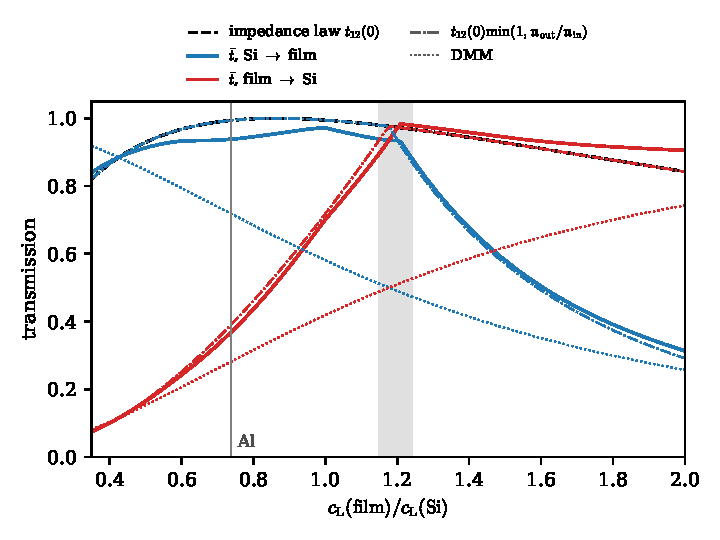
\includegraphics[width=\linewidth]{figures/ch20/limit20_3a.pdf}
\captionof{figure}{Transmission between isotropic silicon and a family of aluminum-like films against the ratio of their longitudinal speeds; the film keeps the density \SI{2.70}{g.cm^{-3}} and the aluminum ratio $c_{\mathrm{T}}/c_{\mathrm{LA}} = 0.498$, and $c_{\mathrm{LA}}(\mathrm{film})/c_{\mathrm{LA}}(\mathrm{Si}) = 0.737$ is aluminum (vertical line). Dashed: the impedance law. Solid: the averages \cref{eq:20.3-avg} from silicon into the film (blue) and back (red). Dash-dot: the leading correction, reciprocity \cref{eq:20.3-recip} applied to the impedance law on the slower side, $t_{12}(0)\min(1, \mathfrak{n}_{\mathrm{out}}/\mathfrak{n}_{\mathrm{in}})$, within \SI{6.9}{\percent} of the averages over the whole range. Dotted: the diffuse mismatch \cref{eq:20.3-dmm}. Gray: speed ratios 1.146 to 1.242, where the impedance law lies within \SI{10}{\percent} of the averages in both directions. In that range $\mathfrak{n}_{\mathrm{film}} \approx \mathfrak{n}_{\mathrm{Si}}$.}\label{fig:20-limit-amm}
\par}
\smallskip
Away from equal interface densities the critical angles of the slower medium's phonons, which the impedance law ignores, remove most of the flux in one direction: for aluminum on silicon the law overstates the escape from the film by a factor 2.70, while reciprocity applied to it, $t_{12}(0)\,\mathfrak{n}_{\mathrm{Si}}/\mathfrak{n}_{\mathrm{Al}} = 0.390$, comes within \SI{6}{\percent} of 0.368.
\end{limitbox}

\subsection{Film absorption and escape time}\label{sec:20.3-escape}

Inside a superconducting film a phonon of energy $E_{\mathrm{ath}}$ above $2\Delta_{\mathrm{BCS}}$ breaks a Cooper pair after a mean free path $\mathfrak{l}_{\mathrm{f}}(E_{\mathrm{ath}})$ (\cref{app:E.12}). Take a film of thickness $d_{\mathrm{f}}$ with a free top face and the substrate below. A phonon that moves at the angle $\theta$ to the normal travels $2d_{\mathrm{f}}/\cos\theta$ between two arrivals at the interface, where it escapes with probability $t_{\mathrm{esc}}$. If it keeps its angle, each round trip is survived with probability $\ee^{-y_{\mathrm{f}}/\cos\theta}$ and ends with an escape with probability $t_{\mathrm{esc}}$. Summing the geometric series of round trips, the probability that the phonon is absorbed before escaping is
\begin{equation}
  P_{\mathrm{abs}}(\theta) = \frac{1 - \ee^{-y_{\mathrm{f}}/\cos\theta}}{1 - (1 - t_{\mathrm{esc}})\,\ee^{-y_{\mathrm{f}}/\cos\theta}} ,
  \qquad y_{\mathrm{f}} = \frac{2d_{\mathrm{f}}}{\mathfrak{l}_{\mathrm{f}}} .
  \label{eq:20.3-pabs-theta}
\end{equation}
A polycrystalline film with a rough top face changes the direction of a phonon at every pass. Each round trip then starts from the flux distribution $2\sin\theta\cos\theta$ of \cref{eq:20.3-avg}, and with $\mu = \cos\theta$ the mean survival over one round trip is
\begin{equation*}
  \int_0^1 2\mu\,\ee^{-y_{\mathrm{f}}/\mu}\,\dd\mu = 2\int_1^\infty\frac{\ee^{-y_{\mathrm{f}}s}}{s^3}\,\dd s = 2E_3(y_{\mathrm{f}}) ,
\end{equation*}
with $s = 1/\mu$ and $E_3$ the exponential integral of order three. The escape probability becomes the average $\bar t_{\mathrm{esc}} = \bar t_{\mathrm{f\to sub}}$ of \cref{eq:20.3-avg}, and the absorption probability per entry is
\begin{equation}
  P_{\mathrm{abs}} = \frac{1 - 2E_3(y_{\mathrm{f}})}{1 - (1 - \bar t_{\mathrm{esc}})\,2E_3(y_{\mathrm{f}})} .
  \label{eq:20.3-pabs}
\end{equation}
For a thin film, $2E_3(y_{\mathrm{f}}) = 1 - 2y_{\mathrm{f}} + O(y_{\mathrm{f}}^2\ln y_{\mathrm{f}})$ and $P_{\mathrm{abs}} \simeq 4d_{\mathrm{f}}/(\mathfrak{l}_{\mathrm{f}}\bar t_{\mathrm{esc}})$: the phonon makes on average $1/\bar t_{\mathrm{esc}}$ round trips of mean length $4d_{\mathrm{f}}$ before it escapes.

The same counting in time gives the escape time. Let the film hold $N_\nu$ phonons of branch $\nu$ per unit volume, distributed isotropically. They strike unit area of the interface at the rate $N_\nu c_\nu/4$, of which the fraction $\langle t_\nu\rangle$, the angle integral in \cref{eq:20.3-avg}, escapes. The film holds $d_{\mathrm{f}}\sum_\nu N_\nu$ phonons per unit area. Let the branches be populated as in equilibrium at a fixed frequency, $N_\nu \propto c_\nu^{-3}$ by \cref{eq:5.2-dosac}. The escape rate is then
\begin{equation*}
  \frac{1}{t_l} = \frac{\sum_\nu N_\nu c_\nu\langle t_\nu\rangle}{4d_{\mathrm{f}}\sum_\nu N_\nu} = \frac{\mathfrak{n}_{\mathrm{f}}\,\bar t_{\mathrm{esc}}}{4d_{\mathrm{f}}\sum_\nu c_\nu^{-3}} .
\end{equation*}
\begin{keyresult}[Film escape time]
A phonon population that is isotropic and mixed among branches leaves a film of thickness $d_{\mathrm{f}}$ at the rate $1/t_l$, with
\begin{equation}
  t_l = \frac{4d_{\mathrm{f}}}{v_s\,\bar t_{\mathrm{esc}}} , \qquad v_s = \frac{\sum_\nu c_\nu^{-2}}{\sum_\nu c_\nu^{-3}} ,
  \label{eq:20.3-tl}
\end{equation}
where $v_s$ is the mean speed of the film's phonons weighted by their density of states and $\bar t_{\mathrm{esc}}$ the mean transmission into the substrate, \cref{eq:20.3-avg}.
\end{keyresult}
\Cref{eq:20.3-tl} assumes that the population is randomized in direction and branch faster than it escapes, that the transmissions are frequency independent, that the top face loses nothing, and that $\bar t_{\mathrm{esc}}$ is the transmission of a clean welded interface, or whatever replaces it. Without the mixing, the \SI{56}{\percent} of the flux beyond the transverse critical angle would never leave, and frequency independence needs wavelengths below $d_{\mathrm{f}}$. With the pair-breaking time $t_{\mathrm{pb}} = \mathfrak{l}_{\mathrm{f}}/v_s$, the thin-film limit of \cref{eq:20.3-pabs} reads $P_{\mathrm{abs}} \simeq t_l/t_{\mathrm{pb}}$, the first term of the competition $t_l/(t_l + t_{\mathrm{pb}})$ between escape and pair breaking.

\begin{workedexample}{Escape from a \SI{60}{nm} aluminum film on silicon}\label{we:20-escape}
The film phonons have $c_{\mathrm{LA}} = 6.63$ and $c_{\mathrm{T}} = \SI{3.30}{km.s^{-1}}$. The sums in \cref{eq:20.3-tl} are $\sum_\nu c_\nu^{-2} = \mathfrak{n}_{\mathrm{Al}} = \SI{0.2062}{s^2.km^{-2}}$ and $\sum_\nu c_\nu^{-3} = \SI{0.0590}{s^3.km^{-3}}$, so $v_s = \SI{3.50}{km.s^{-1}}$, close to the transverse speed because transverse modes dominate the density of states.

The escape probability is the average from aluminum into silicon. The acoustic mismatch model gives $\bar t_{\mathrm{esc}} = 0.368$, from 0.624 for longitudinal, 0.313 for SV and 0.359 for SH phonons; the diffuse mismatch model gives 0.282. With $d_{\mathrm{f}} = \SI{60}{nm}$,
\begin{equation*}
  t_l = \frac{4\times\SI{60}{nm}}{\SI{3.50}{km.s^{-1}}\times0.368} = \SI{0.187}{ns} \quad\text{(acoustic)}, \qquad \SI{0.244}{ns} \quad\text{(diffuse)},
\end{equation*}
a factor 1.31 between the two models. Near $2\Delta_{\mathrm{BCS}}$ a phonon in aluminum breaks a pair in the time $t_0 \approx \SI{0.26}{ns}$, the characteristic phonon lifetime of Kaplan and coworkers~\cite{kaplan1976quasiparticle}, \cite[p.~2]{guruswamy2014quasiparticle}, which \cref{sec:20.4} defines as the pair-breaking time at threshold. Hence $t_l/t_0 = 0.72$ (acoustic) or 0.94 (diffuse). A \SI{60}{nm} film loses its phonons about as fast as they break pairs, which is the regime in which \cref{sec:20.4} finds the quasiparticle yield sensitive to $t_l/t_0$. If the mean free path were $\mathfrak{l}_{\mathrm{f}} = v_st_0 = \SI{0.909}{\micro m}$, then $y_{\mathrm{f}} = 0.132$ and \cref{eq:20.3-pabs} would give $P_{\mathrm{abs}} = 0.422$, against $t_l/(t_l + t_0) = 0.418$.
\end{workedexample}

\subsection{The fitted silicon-to-aluminum coefficient}\label{sec:20.3-fit}

Martinez and coworkers illuminated the back of silicon wafers 300 to \SI{380}{\micro m} thick, \SI{2}{cm} square, that carried \SI{60}{nm} aluminum resonators. They compared the measured phonon pulses with a Monte Carlo simulation using specular reflection, and the silicon-to-aluminum coefficient that reproduced the data lay between 0.30 and 0.55~\cite[Sect.~V]{martinez2019measurements}. Their simulation does not propagate phonons inside the aluminum. A phonon that crosses produces a signal with the pair-breaking efficiency or is removed, and the fitted coefficient's complement includes phonons that enter the film and come back~\cite[Sect.~IV]{martinez2019measurements}. The fitted coefficient is therefore the probability that a phonon arriving from silicon is absorbed in the film,
\begin{equation}
  T_{\mathrm{fit}} = \bar t_{\mathrm{Si\to Al}}\,P_{\mathrm{abs}} .
  \label{eq:20.3-Tfit}
\end{equation}
With the acoustic-mismatch value 0.938, the fit gives $P_{\mathrm{abs}} = 0.320$ to 0.586. Inverting \cref{eq:20.3-pabs} with $\bar t_{\mathrm{esc}} = 0.368$ gives $\mathfrak{l}_{\mathrm{f}}/d_{\mathrm{f}} = 23.1$ to 8.3, or $\mathfrak{l}_{\mathrm{f}} = 1.39$ to \SI{0.50}{\micro m}, and $t_{\mathrm{pb}} = \mathfrak{l}_{\mathrm{f}}/v_s = 0.40$ to \SI{0.14}{ns}, the same order as $t_0$. Keeping the angle of each phonon instead, \cref{eq:20.3-pabs-theta} averaged with $t_{\mathrm{esc}} = \bar t_{\mathrm{esc}}$ gives 1.29 to \SI{0.46}{\micro m}; the diffuse-mismatch pair, 0.718 and 0.282, gives 1.19 to \SI{0.31}{\micro m}. The fit thus constrains the pair-breaking length over the thickness, $\mathfrak{l}_{\mathrm{f}}/d_{\mathrm{f}} \approx 5$ to 23 across both models, and says little about the interface. In the thin-film limit $T_{\mathrm{fit}} \to (\mathfrak{n}_{\mathrm{Al}}/\mathfrak{n}_{\mathrm{Si}})\,4d_{\mathrm{f}}/\mathfrak{l}_{\mathrm{f}}$ for any interface that conserves energy, by reciprocity (\cref{eq:20.3-pabs,eq:20.3-recip}), and the interface model enters only through the finite-thickness corrections. Read as a transmission, the fit would put the escape probability at $(\mathfrak{n}_{\mathrm{Si}}/\mathfrak{n}_{\mathrm{Al}})\times(0.30$ to $0.55) = 0.118$ to 0.216 by \cref{eq:20.3-recip}, below both models. The inferred lengths are estimates: they inherit the specular, mode-conserving simulation of the fit and the isotropic averages of this section. An earlier silicon detector model matched its data with a \SI{33}{\percent} probability for a phonon to be absorbed at an amorphous-silicon/aluminum interface, the rest scattering back diffusely~\cite[Sect.~III\,G]{leman2012invited}; that coefficient is an absorption probability of the same kind.

\subsection{Anisotropy and interlayers}\label{sec:20.3-aniso}

The isotropic averages hide the anisotropy of silicon, whose longitudinal speed ranges from 8.43 to \SI{9.35}{km.s^{-1}} and whose transverse speeds from 4.67 to \SI{5.84}{km.s^{-1}} (\cref{eq:C.18-cubic}). Giving the isotropic silicon its $[100]$ speeds, 8.43 and \SI{5.84}{km.s^{-1}}, or its $[111]$ speeds, 9.35 and \SI{5.09}{km.s^{-1}}, moves $\bar t_{\mathrm{esc}}$ from 0.368 to 0.327 and 0.405, and $t_l$ for \SI{60}{nm} from 0.187 to 0.210 and \SI{0.169}{ns}; $\bar t_{\mathrm{Si\to Al}}$ moves only between 0.927 and 0.943. These are sensitivities, not bounds. The texture of the film matters less, since it changes the longitudinal speed of aluminum by at most \SI{3}{\percent} (\cref{app:C.18}). In the anisotropic problem the critical angles depend on the direction in the interface plane, the group velocity is not parallel to $\vect{Q}$, and the plane waves on each side follow from the Christoffel equation \cref{eq:C.18-christoffel}; the boundary problem becomes six by six. The reciprocity \cref{eq:20.3-recip} holds there unchanged.

Real interfaces carry a native oxide or a deposited amorphous layer a few nanometers thick. A flat layer that does not dissipate cannot change which waves propagate in silicon, since $Q_\parallel$ is conserved through every layer: the critical angles and the \SI{56}{\percent} of trapped film flux stay as they are. The layer changes the transmission inside the cone. At normal incidence take a layer of impedance $Z_{\mathrm{ac},3}$, speed $c_3$ and thickness $h$. At the quarter-wave frequency $c_3/4h$ the wave crosses it with the phase $\pi/2$, and the layer maps the particle velocity $\dot u$ and the force $-\sigma_{zz}$ at its far face onto $\ii(-\sigma_{zz})/Z_{\mathrm{ac},3}$ and $\ii Z_{\mathrm{ac},3}\dot u$ at its near face. A medium of impedance $Z_{\mathrm{ac},2}$ behind it then looks like one of impedance $Z_{\mathrm{ac},3}^2/Z_{\mathrm{ac},2}$, and \cref{eq:C.18-transmission} with this replacement gives the lowest transmission,
\begin{equation*}
  t_{\min} = \frac{4Z_{\mathrm{ac},1}Z_{\mathrm{ac},2}Z_{\mathrm{ac},3}^2}{\bigl(Z_{\mathrm{ac},1}Z_{\mathrm{ac},2} + Z_{\mathrm{ac},3}^2\bigr)^2} ,
\end{equation*}
since the transmission oscillates between this value and the bare $t_{12}(0)$ as the frequency varies. Amorphous SiO$_2$, with $\rho_T = \SI{2.2}{g.cm^{-3}}$ and $\rho_Tc_{\mathrm{LA}}^2 = \SI{7.40e10}{Pa}$ (\cref{sec:16.7}), has $c_{\mathrm{LA}} = \SI{5.80}{km.s^{-1}}$ and $Z_{\mathrm{ac}} = \SI{12.8e6}{kg.m^{-2}.s^{-1}}$. Between silicon and aluminum it gives $t_{\min} = 0.844$, against 0.994 without the layer, at \SI{0.72}{THz} for a \SI{2}{nm} layer; a \SI{1}{nm} layer transmits 0.901 at \SI{0.8}{THz}. A rough or disordered layer scatters diffusely instead, does not conserve $Q_\parallel$, and can release trapped modes; the diffuse mismatch model is the limit of complete randomization. Until the escape probability of a real film is measured, the spread from 0.282 to 0.368, a factor 1.31 in $t_l$, is the uncertainty to carry.
